\documentclass[xcolor=dvipsnames]{beamer}
\usepackage[T1]{fontenc}
\usepackage[utf8]{inputenc}
\usepackage[english,slovak]{babel}

\usepackage{amsmath}
\usepackage{amsthm}
\usetheme{Pittsburgh}
\useoutertheme{shadow}

\usepackage{graphicx}
\usepackage{caption}
\usepackage{subcaption}

\usepackage[]{algorithm2e}
\usepackage{listings}
 \setbeamercovered{transparent}
 \usepackage{cuted}
\usepackage[export]{adjustbox}
\usepackage{mathtools}

\usepackage{lipsum}

\newcommand\Wider[2][3em]{%
\makebox[\linewidth][c]{%
  \begin{minipage}{\dimexpr\textwidth+#1\relax}
  \raggedright#2
  \end{minipage}%
  }%
}





\usetheme{Warsaw}

\setbeamercolor{normal text}{fg=white,bg=black!90}
\setbeamercolor{structure}{fg=white}

\setbeamercolor{alerted text}{fg=red!85!black}

\setbeamercolor{item projected}{use=item,fg=black,bg=item.fg!35}

\setbeamercolor*{palette primary}{use=structure,fg=structure.fg}
\setbeamercolor*{palette secondary}{use=structure,fg=structure.fg!95!black}
\setbeamercolor*{palette tertiary}{use=structure,fg=structure.fg!90!black}
\setbeamercolor*{palette quaternary}{use=structure,fg=structure.fg!95!black,bg=black!80}

\setbeamercolor*{framesubtitle}{fg=white}

\setbeamercolor*{block title}{parent=structure,bg=black!60}
\setbeamercolor*{block body}{fg=black,bg=black!10}
\setbeamercolor*{block title alerted}{parent=alerted text,bg=black!15}
\setbeamercolor*{block title example}{parent=example text,bg=black!15}





%-------------------------------------------------------------------------------------
\title{\bf Deep neural network on Arduino}
\author{Michal CHOVANEC, PhD}


%\setbeamertemplate{footline}[frame number]{}
\setbeamertemplate{navigation symbols}{}


\date[EURP]{}
\begin{document}

\begin{frame}
\titlepage


\begin{columns}
\begin{column}{0.5\textwidth}

  \begin{figure}
    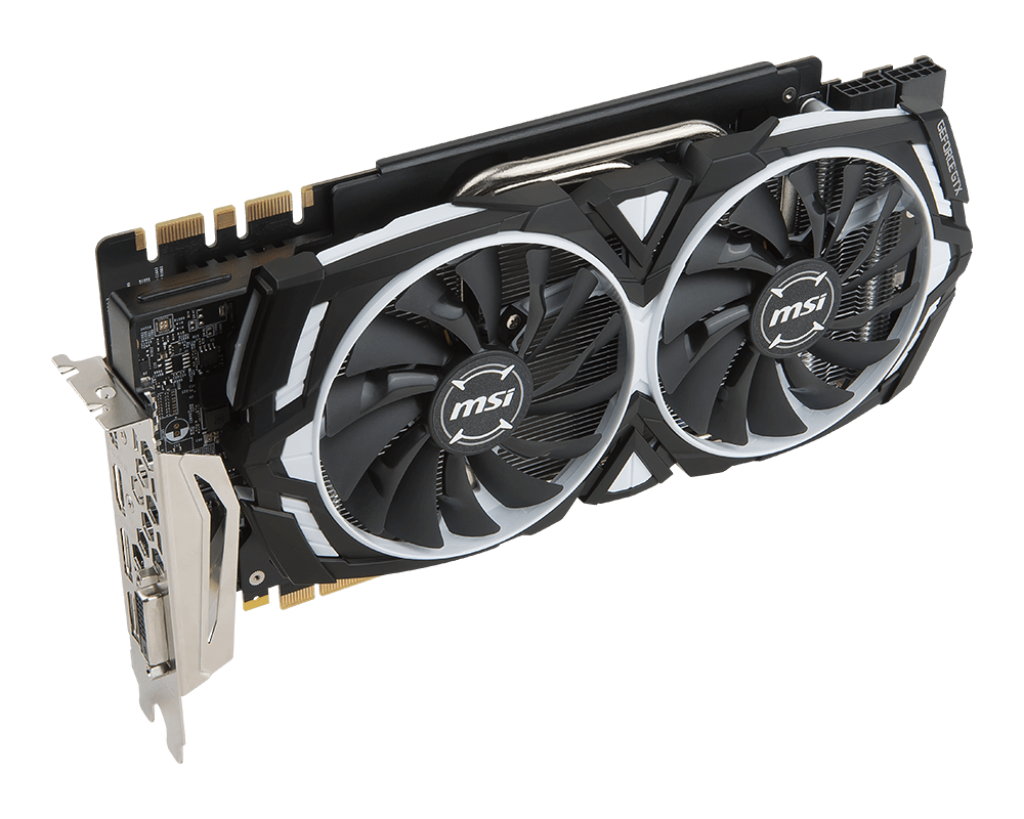
\includegraphics[scale=0.15]{gpu.png}
  \end{figure}

\end{column}
\begin{column}{0.5\textwidth}  %%<--- here

  \begin{figure}
  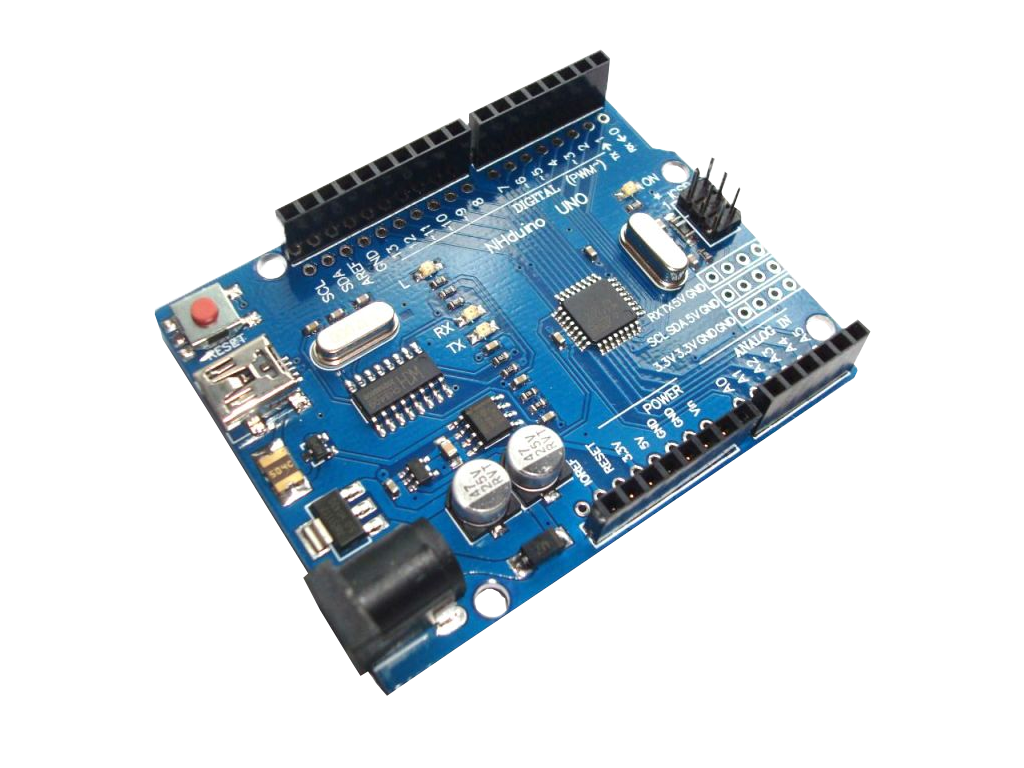
\includegraphics[scale=0.1]{arduino.png}
  \end{figure}

\end{column}
\end{columns}

\end{frame}


\begin{frame}{\bf Goal}

Train deep neural network on GPU and run it on Arduino

\begin{itemize}
  \item Dataset MNIST handwritten digits down sampled from 28x28 to 9x9 pixels
  \item Fully connected network with two hidden ReLU layers
\end{itemize}


\begin{columns}
\begin{column}{0.5\textwidth}

  \begin{figure}
    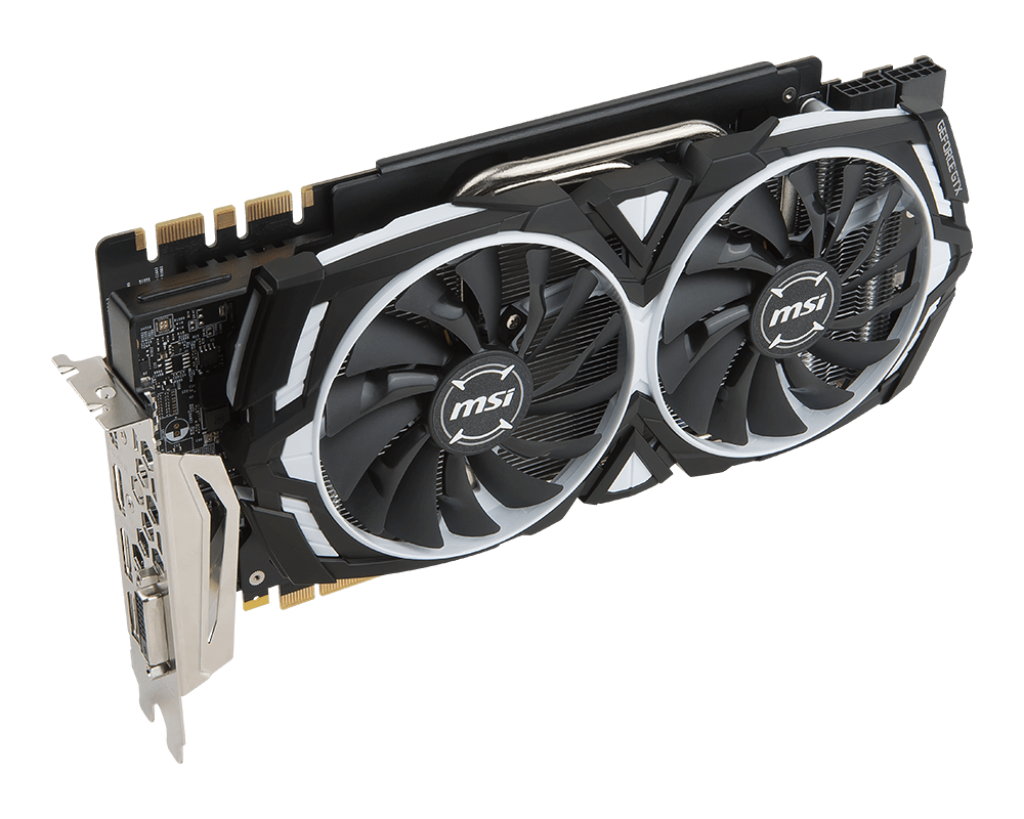
\includegraphics[scale=0.15]{gpu.png}
  \end{figure}

\end{column}
\begin{column}{0.5\textwidth}  %%<--- here

  \begin{figure}
  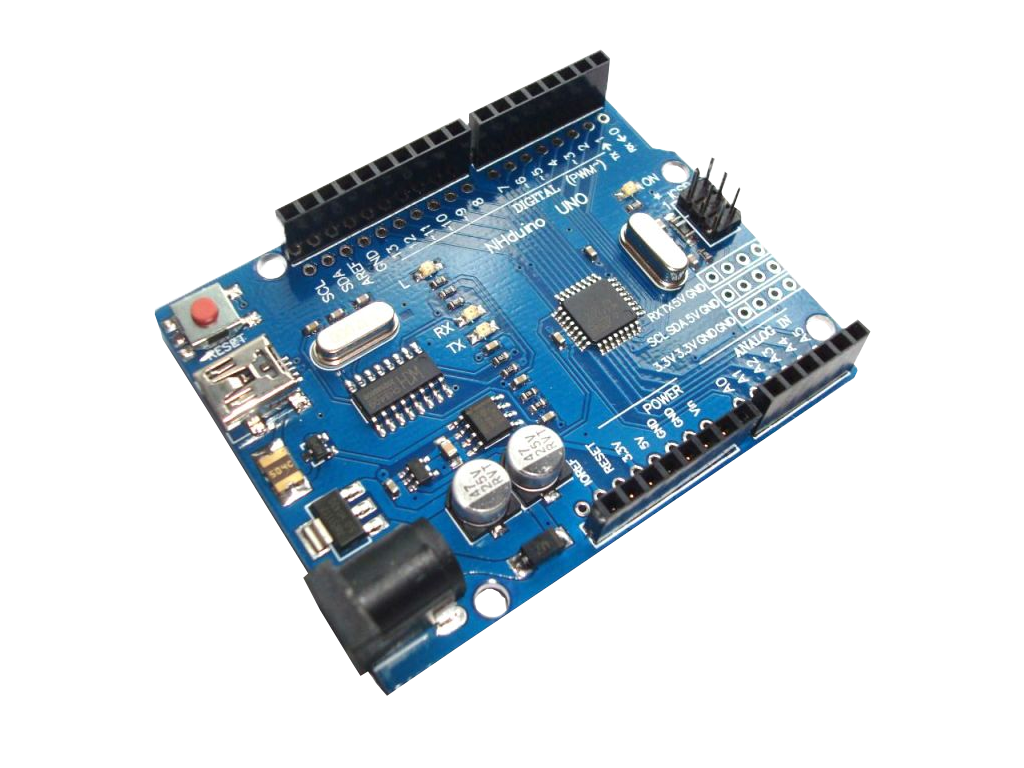
\includegraphics[scale=0.1]{arduino.png}
  \end{figure}

\end{column}
\end{columns}


\end{frame}



\begin{frame}{\bf Network topology}

\begin{figure}
  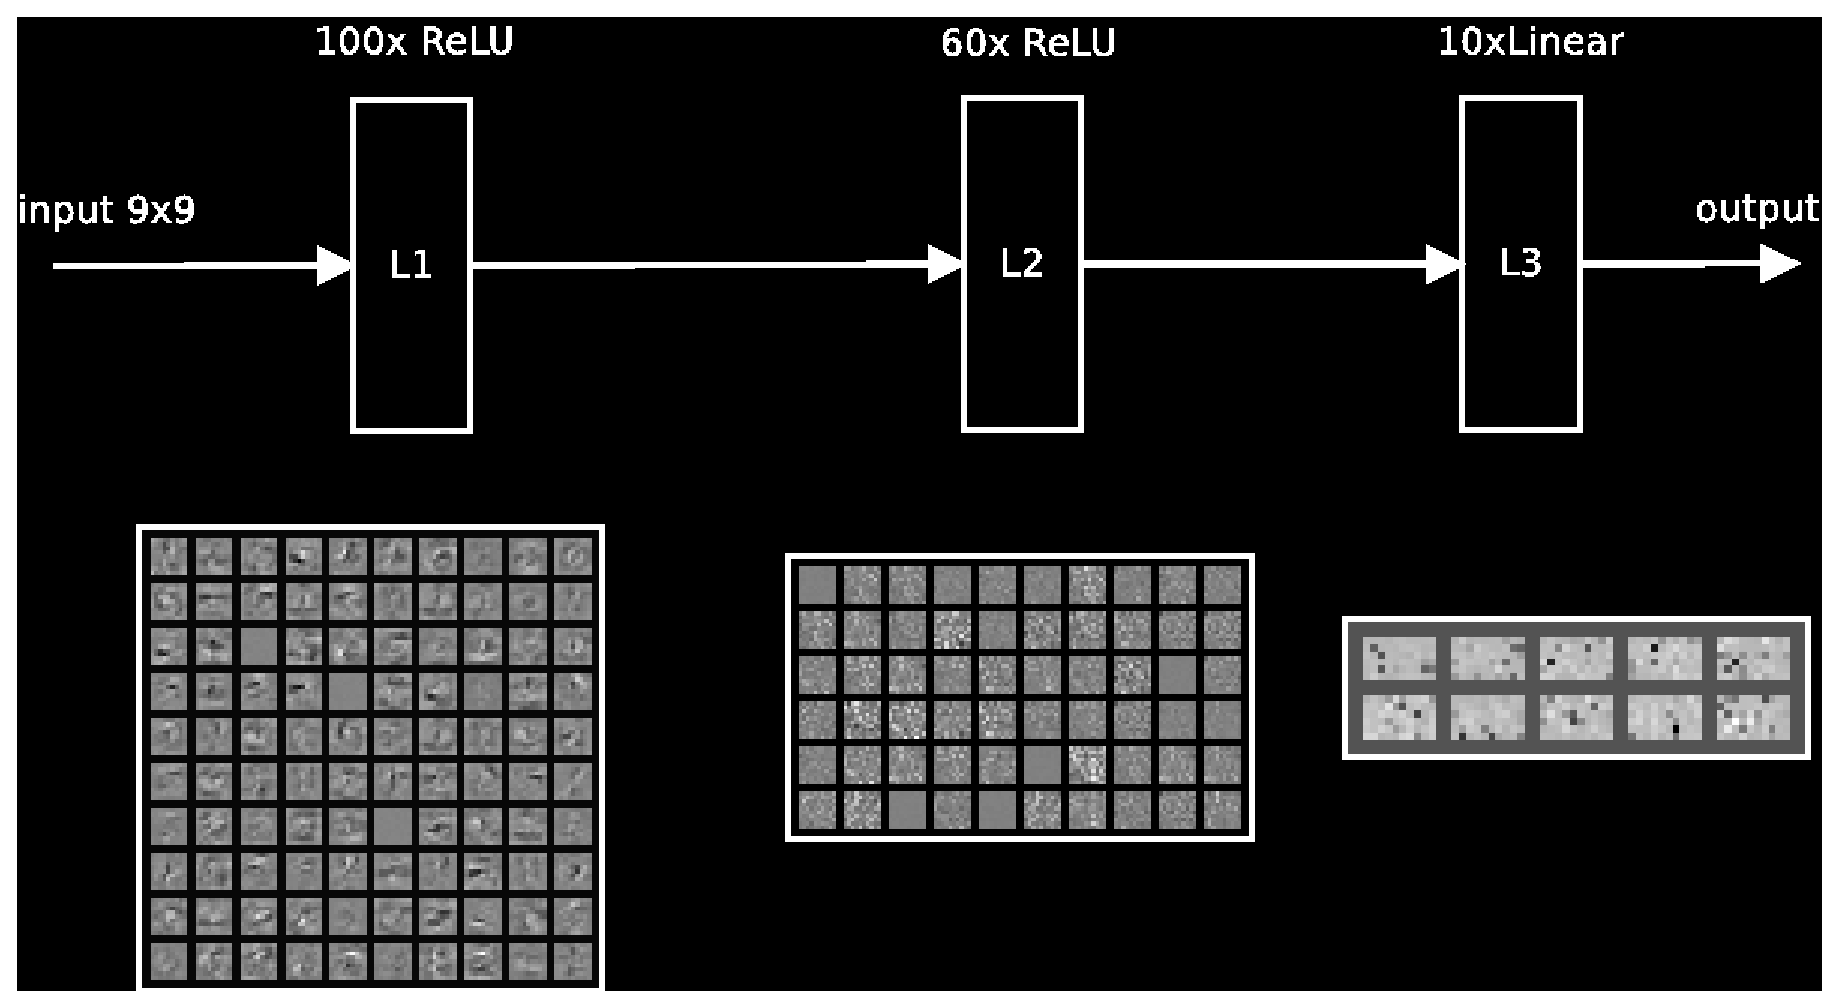
\includegraphics[width=\linewidth]{nn_topology_trained_black.eps}
\end{figure}

\end{frame}

\begin{frame}

\centering {\bf Training on GPU (1080ti)}

\end{frame}


\begin{frame}[fragile]
\frametitle{\bf Converting weights}

use simple linear mapping : \\
\begin{align*}
  w_{int} &= 127\frac{w_{float}}{w_{max}} \\
  scaling\_factor &= 1000w_{max}
\end{align*}
\bigskip
  \lstset{language=C++}
\begin{lstlisting}
  #define layer_1_scaling_factor  515

  signed char weights_layer_1[8200]={
  -34, -17, -4, 18, 24, -9, 8, -7 ... };
\end{lstlisting}

\end{frame}



\begin{frame}[fragile]
\frametitle{\bf Layer kernel}

{\tiny
  \lstset{language=C++}
\begin{lstlisting}
void matrix_vector_dot_kernel(t_nn_buffer *output, t_nn_buffer *input,
                              signed char *weights,
                              unsigned int input_size,
                              unsigned int output_size,
                              unsigned int weights_scaling)
{
  unsigned int w_ptr = 0;
  for (unsigned int j = 0; j < output_size; j++) {
    unsigned int input_ptr  = 0;
    unsigned int size       = input_size+1;

    long int sum = 0;

    while (size >= 4) {
      sum+= (weights[w_ptr]*input[input_ptr]); w_ptr++; input_ptr++;
      sum+= (weights[w_ptr]*input[input_ptr]); w_ptr++; input_ptr++;
      sum+= (weights[w_ptr]*input[input_ptr]); w_ptr++; input_ptr++;
      sum+= (weights[w_ptr]*input[input_ptr]); w_ptr++; input_ptr++;

      size-= 4;
    }

    while (size) {
      sum+= (weights[w_ptr]*input[input_ptr]); w_ptr++; input_ptr++;
      size--;
    }

    sum = (sum*weights_scaling)/(127*1000);
    output[j] = sum;
  }
}
\end{lstlisting}
}

\end{frame}


\begin{frame}

\centering {\bf Testing network on CPU}

\end{frame}

\begin{frame}{\bf Floating point vs fixed point result}

{\tiny
32 bit floating point confusion matrix :
% Please add the following required packages to your document preamble:
% \usepackage[table,xcdraw]{xcolor}
% If you use beamer only pass "xcolor=table" option, i.e. \documentclass[xcolor=table]{beamer}
\begin{table}[]
\centering
\label{my-label}
\begin{tabular}{llllllllll}
967                                     & 0                                       & 6               & 0               & 0               & 3               & 6               & 1               & 6               & 4               \\
0                                       & 1126                                    & 0               & 0               & 1               & 2               & 3               & 12              & 2               & 5               \\
1                                       & 3                                       & 1000            & 5               & 3               & 1               & 1               & 13              & 4               & 0               \\
2                                       & 2                                       & 3               & 979             & 0               & 17              & 1               & 1               & 5               & 7               \\
0                                       & 0                                       & 2               & 0               & 942             & 2               & 2               & 3               & 6               & 15              \\
2                                       & 0                                       & 2               & 9               & 0               & 852             & 5               & 1               & 7               & 6               \\
6                                       & 1                                       & 4               & 0               & 10              & 8               & 938             & 0               & 2               & 1               \\
1                                       & 1                                       & 10              & 9               & 1               & 1               & 0               & 986             & 5               & 6               \\
1                                       & 2                                       & 5               & 7               & 1               & 3               & 1               & 1               & 933             & 3               \\
0                                       & 0                                       & 0               & 1               & 24              & 3               & 0               & 10              & 4               & 962             \\
\textbf{98.673}                         & \textbf{99.207}                         & \textbf{96.899} & \textbf{96.931} & \textbf{95.927} & \textbf{95.516} & \textbf{98.015} & \textbf{95.914} & \textbf{95.791} & \textbf{95.342} \\
{\color[HTML]{FE0000} \textbf{result=}} & {\color[HTML]{FE0000} \textbf{96.86\%}} &                 &                 &                 &                 &                 &                 &                 &
\end{tabular}
\end{table}


8 bit fixed point confusion matrix :

% Please add the following required packages to your document preamble:
% \usepackage[table,xcdraw]{xcolor}
% If you use beamer only pass "xcolor=table" option, i.e. \documentclass[xcolor=table]{beamer}
\begin{table}[]
\centering
\label{my-label}
\begin{tabular}{llllllllll}
967                                      & 0                                       & 5               & 0               & 1               & 3               & 6               & 1               & 6               & 4               \\
0                                        & 1126                                    & 0               & 0               & 1               & 1               & 3               & 11              & 2               & 5               \\
1                                        & 3                                       & 1001            & 5               & 3               & 1               & 1               & 13              & 2               & 0               \\
2                                        & 2                                       & 3               & 976             & 0               & 15              & 1               & 1               & 5               & 7               \\
0                                        & 0                                       & 2               & 0               & 943             & 2               & 1               & 3               & 5               & 16              \\
2                                        & 0                                       & 2               & 11              & 0               & 856             & 6               & 1               & 9               & 7               \\
6                                        & 1                                       & 4               & 0               & 8               & 6               & 938             & 0               & 2               & 1               \\
1                                        & 1                                       & 10              & 9               & 1               & 1               & 0               & 989             & 3               & 7               \\
1                                        & 2                                       & 5               & 9               & 1               & 4               & 1               & 1               & 936             & 4               \\
0                                        & 0                                       & 0               & 0               & 24              & 3               & 0               & 8               & 4               & 958             \\
\textbf{98.673}                          & \textbf{99.207}                         & \textbf{96.996} & \textbf{96.634} & \textbf{96.029} & \textbf{95.964} & \textbf{98.015} & \textbf{96.206} & \textbf{96.099} & \textbf{94.945} \\
{\color[HTML]{FE0000} \textbf{result =}} & {\color[HTML]{FE0000} \textbf{96.91\%}} &                 &                 &                 &                 &                 &                 &                 &
\end{tabular}
\end{table}
}

\end{frame}


\begin{frame}

\centering {\bf Running on Arduino}

\end{frame}

\begin{frame}{\bf Running on Arduino}

1000 random samples from testing set

{\tiny
% Please add the following required packages to your document preamble:
% \usepackage[table,xcdraw]{xcolor}
% If you use beamer only pass "xcolor=table" option, i.e. \documentclass[xcolor=table]{beamer}
\begin{table}[]
\centering
\begin{tabular}{llllllllll}
97                                                                 & 0                                      & 0              & 0               & 0               & 0               & 0            & 0              & 0              & 1               \\
0                                                                  & 117                                    & 0              & 0               & 0               & 0               & 0            & 3              & 0              & 0               \\
0                                                                  & 1                                      & 96             & 0               & 0               & 0               & 0            & 2              & 0              & 0               \\
0                                                                  & 1                                      & 1              & 95              & 0               & 2               & 0            & 0              & 0              & 0               \\
0                                                                  & 0                                      & 0              & 0               & 82              & 0               & 0            & 0              & 0              & 1               \\
0                                                                  & 0                                      & 1              & 2               & 0               & 81              & 0            & 0              & 1              & 2               \\
1                                                                  & 0                                      & 1              & 0               & 0               & 1               & 95           & 0              & 0              & 1               \\
0                                                                  & 0                                      & 0              & 1               & 0               & 0               & 0            & 111            & 0              & 0               \\
0                                                                  & 0                                      & 0              & 0               & 0               & 0               & 0            & 0              & 97             & 0               \\
0                                                                  & 0                                      & 0              & 0               & 3               & 1               & 0            & 0              & 0              & 102             \\
\textbf{98.98}                                                     & \textbf{98.319}                        & \textbf{96.97} & \textbf{96.939} & \textbf{96.471} & \textbf{95.294} & \textbf{100} & \textbf{95.69} & \textbf{98.98} & \textbf{95.327} \\
{\color[HTML]{FE0000} \textbf{result =}}                           & {\color[HTML]{FE0000} \textbf{97.3\%}} &                &                 &                 &                 &              &                &                &                 \\
\textbf{\begin{tabular}[c]{@{}l@{}}time per\\ sample\end{tabular}} & \textbf{0.487s}                        &                &                 &                 &                 &              &                &                &
\end{tabular}
\end{table}
}

\begin{figure}
  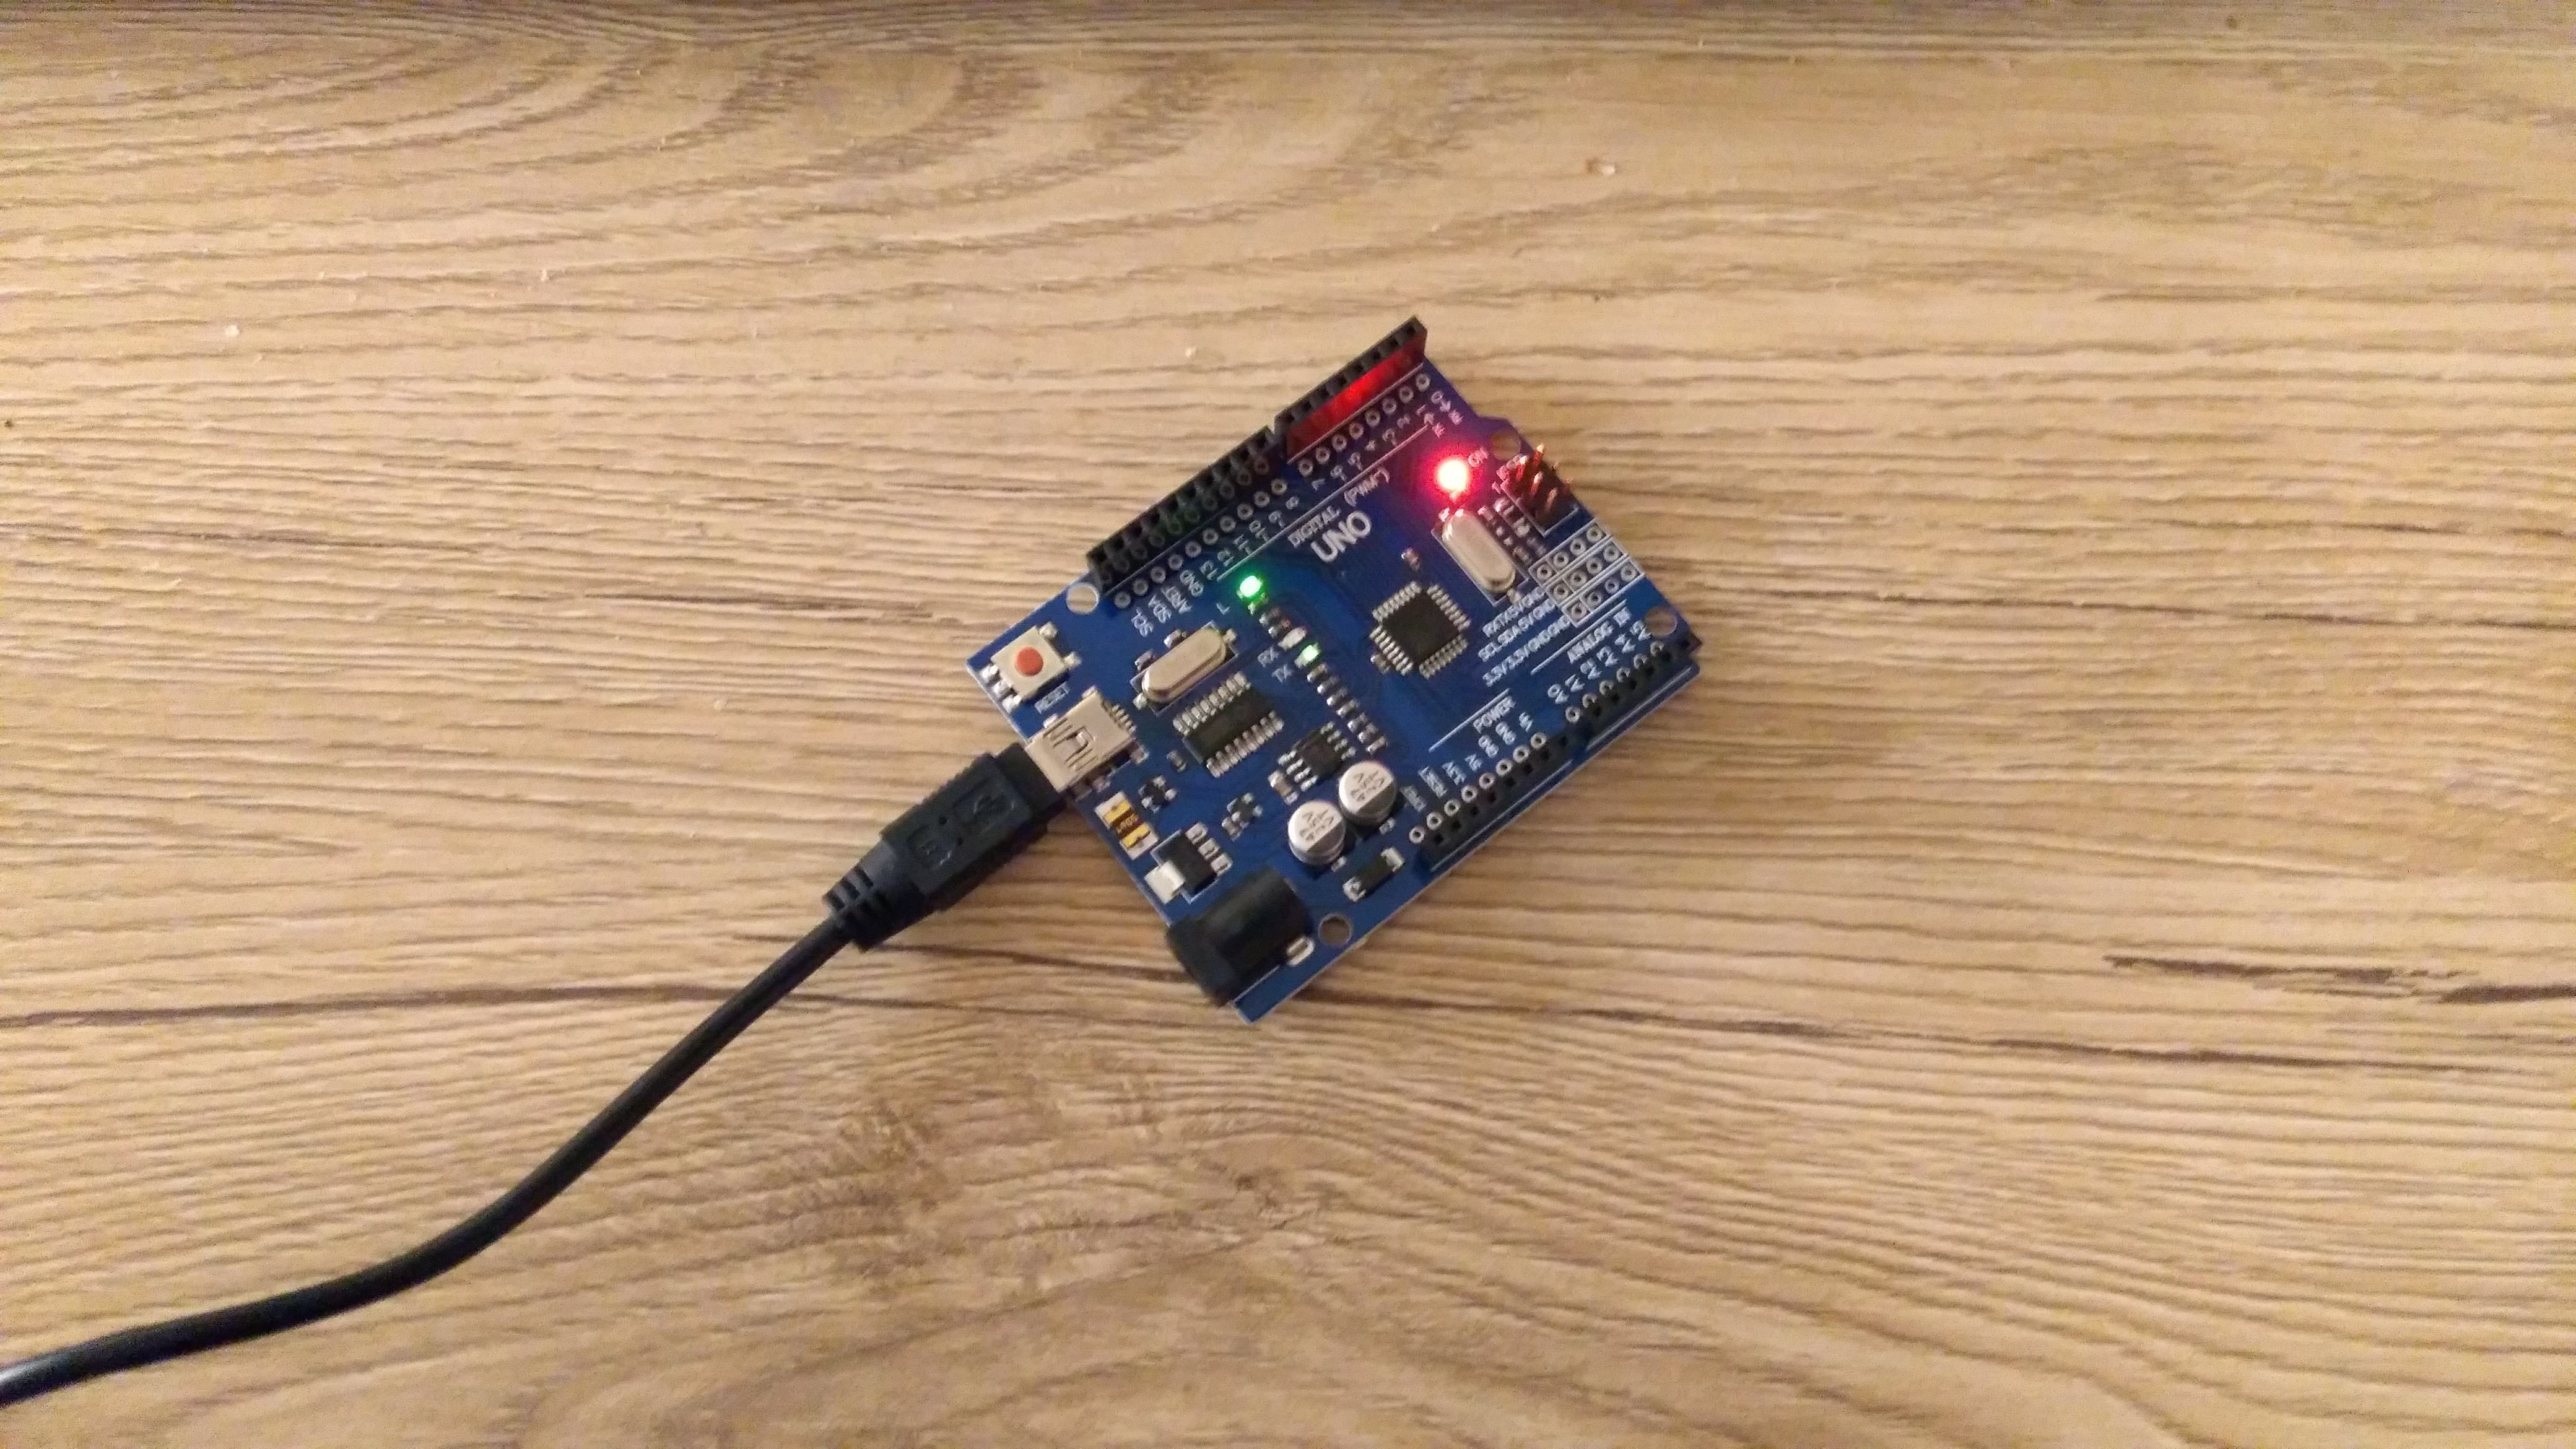
\includegraphics[scale=0.03]{setup.jpg}
\end{figure}

\end{frame}

\end{document}
